In this section, first the approaches of the IKC and TM frameworks towards interval representation are compared. Next, their approaches towards the evaluation of Allen relationships between a crisp interval and an interval subject to uncertainty are compared.

\subsection{\label{subsec:comp-interval}Comparison of Approaches to Interval Representation}
The IKC framework uses IKTI to represent time intervals subject to uncertainty, whereas the TM framework uses UTI for this. In both approaches, to consider uncertainty about the exact CTI which is intended, uncertainty about the exact starting and ending instants of the intended interval is considered and confidence in the context of this uncertainty is expressed using two possibility distributions. In an IKTI, these possibility distributions each define one IKV. One of these then defines the IKTI's starting instant and the other defines its ending instant. In an UTI, one of these possibility distributions is directly meant to define the UTI's starting instant and the other is directly meant to define the UTI's ending instant. It is obvious that the concepts of IKTI and UTI are exactly the same, except for the explicit usage of the concept of IKV in IKTI to define and describe uncertainty about starting and ending instants. This equality implies that both approaches have the same basic restriction: they cannot represent every kind of interval subject to uncertainty imaginable. For example, imagine an ordered set of instants coinciding with $\mathbb{N}_0$ and imagine an interval subject to uncertainty in this set, where the intended interval is either $\left[2, 4\right]$ (possibility $1$) or $\left[3, 7\right]$ (possibility $1$). This interval can not be modelled by a combination of possibility distributions defining the starting and ending instants without making $\left[2, 7\right]$ and $\left[3, 4\right]$ also possible as intended intervals to some extent. This issue was first suggested about IKTI in~\cite{Billiet2012}.

Now, a major difference between the two frameworks, concerning their approaches towards the representation of time intervals in general, is that the TM framework includes visualization in its approach.

A first consequence of this is that the TM framework allows the visualization of multiple CTI in the same image plane. In theory, it should also allow the visualization of multiple UTI in the same image plane. However, if the interval space area's visualizing these UTI overlap, it is not yet researched which greyscale (or other) color and intensity each interval point in this overlapping area should have, as the appearance of such interval point should both reflect the possibility of it being the interval intended by the one UTI and the possibility of it being the interval intended by the other UTI. The advantage of the ability to visualize multiple time intervals in the same image plane is that a human observer could easily assess certain characteristics of a distribution of time intervals from an image containing their visualization. The IKC framework, on the other hand, doesn't incorporate any form of visualization and doesn't allow such human assessments.

A second consequence of this is that the TM framework requires that an UTI can be visualized, using a visualization method which actually visualizes the possibility of a CTI of being the interval intended by this UTI for every CTI that has a non-zero possibility of this. Thus, a method is required, to calculate the possibility of a given CTI of being the interval intended by an UTI based on the possibility distributions defining this UTI. This method is found by demanding that the given CTI's starting instant is the intended interval's starting instant \emph{and} that the given CTI's ending instant is the intended interval's ending instant and by determining the possibility of the conjunction of both demands using the standard possibility theory conjunction operator `minimum'. Although not necessary for the correct and consistent functioning of the TM framework, it appears to be the intention of the TM framework that possibility about the exact starting or ending instant of the interval intended by the UTI could be derived from the possibility distribution defining the possibility that a given CTI is the interval intended by the UTI. For this derivation to be consistent, the possibility distributions defining the UTI must be convex. Given an ordered set $T$ and an UTI $J = (\pi_{J_s}, \pi_{J_e})$ in $T$ with possibility $\pi_J(I)$ that a given CTI $I = \left[s_i, e_i\right]$ is the exact time interval intended by $J$, the derivations can be calculated as follows:

\begin{align}
\pi_{J_s}(s_i) = \max_{K = \left[s_i, k\right], k \in T, k > s_i}(\pi_J(K)) \nonumber \\
\pi_{J_e}(e_i) = \max_{K = \left[k, e_i\right], k \in T, k < e_i}(\pi_J(K)) \nonumber
\end{align}

With respect to this convexity demand, the IKC framework is similar: the possibility distributions defining the starting and ending IKV of an IKTI are also demanded to be convex by the IKC framework, although this appears not to be necessary for the framework to function correctly and consistently.

\subsection{\label{subsec:comp-eval}Comparison of Approaches to Allen Relationship Evaluation}
As mentioned before, a major difference between the two frameworks, concerning their approaches towards the representation of time intervals in general, is that the TM framework includes visualization in its approach. As a result, it also includes visualization in its approach towards the evaluation of Allen relationships between a CTI and an UTI.

A first consequence of this is that, given a CTI, an UTI, its URZ and their visualizations in the same image, the TM framework allows a visual, human assessment of the degree of possibility of this CTI being in an Allen relationship with this UTI, for every Allen relationship with a non-zero such degree, based on this image. Moreover, those with possibility degree equal to zero can be easily found before any calculation is done: they are the relationships not contained in the set corresponding to the URZ containing the CTI's interval point. On the other hand, to examine the respective possibilities of a given CTI of being in several different Allen relationships with a given IKTI using the IKC framework, a new collection of specific IKC and a specific aggregation of these should be constructed for every Allen relationship under consideration, allowing to calculate its exact possibility and necessity. In contrast to the TM framework, using the IKC framework a human assessment before any calculation is not possible and it is not known before any calculation which Allen relationships will result in a possibility degree equal to zero.

A second consequence is that, given an UTI and its URZ, multiple CTI can be visualized in the same image as the UTI and its URZ. Thus, the same image could provide a visual, human assessment of the possibilities with which multiple CTI are in Allen relationships with the UTI, before any calculation is done. Again, the IKC framework would need a different collection of specific IKC and a specific aggregation of these for every Allen relationship under consideration, but calculating the possibilities for several CTI to be in a given Allen relationship with a given IKTI would not provide much extra work.

A third consequence is that, in the TM framework, given an UTI, its URZ and a visualization of these in the same image, a given Allen relationship could correspond with several URZ. Thus, given a distribution of CTI, it is not easy to visually assess which CTI have a non-zero possibility of being in the given Allen relationship with the given UTI. On the other hand, assessing this using the IKC framework is impossible without any calculation, but the necessary calculations are pretty straightforward.

Although this has not been rigorously researched yet, it is the conviction of the authors that a great strength of the IKC framework lies in its modular approach towards the evaluation of temporal relationships, resulting in a flexibility and an easy handling of complex temporal relationships, while the visualization of these using the TM framework could become complex and heavy. This would give the IKC framework a major advantage over the TM framework, when used in reasoning systems like e.g. decision support systems. Moreover, in some cases the visualization step used in the TM framework could be a redundant step.

%Both above statements say something about `visual assessment'. However, to actually calculate the plausibilities in question, the IKC framework requires a rather complex numerical (?) calculation based on the set of IKC and its combination corresponding to the Allen relationship and the CTI in question. In this, the TM framework is similar, as it also requires a rather complex geometrical construction and a calculation based on this, for every Allen relationship and CTI in question, IF the crisp interval point is in an URZ corresponding with a non-singleton set of Allen relationships. Else, the plausibility for the Allen relationship in the singleton is 1, all others are 0.

%Although it has not been rigorously researched yet, it is the conviction of the authors that both frameworks can also be used to evaluate combinations of Allen relationships between crisp intervals and an UTI/IKTI. For example: `what is the possibility that $J$ is before $K$ but after $I$?'.

\subsection{\label{subsec:example}An Example}
In this section, some of the comparison results presented above will be illustrated using a simple example.

\begin{example}
Consider an ordered set of instants $T$ coinciding with $\mathbb{R}$, a CTI $I = \left[1, 3\right]$ and a time interval $J$ of which the starting instant is defined by a triangular possibility distribution on $T$ with core $\{5\}$ and support $\left[2, 7\right]$ and of which the ending instant is defined by a triangular possibility distribution on $T$ with core $\{12\}$ and support $\left[9, 15\right]$. The visualization of this example situation using the TM framework is shown in figure \ref{fig:ex}. The interval point for $I$ lies in the URZ `PM'. Thus, possibility is higher than zero for $I$ to be in a `meets', `before', or `overlaps' relationship with $J$. As the darkest point in the `overlaps' area part is very light, the darkest point in the `meets' line segment is reasonably dark and the darkest point in the `before' area part is perfectly black, it can be estimated that $I$ overlaps $J$ with a low possibility, $I$ meets $J$ with a high but non-zero possibility and $I$ is before $J$ with possibility $1$.

TODO: IKC

\end{example}

\begin{figure}[h]
	\centering
	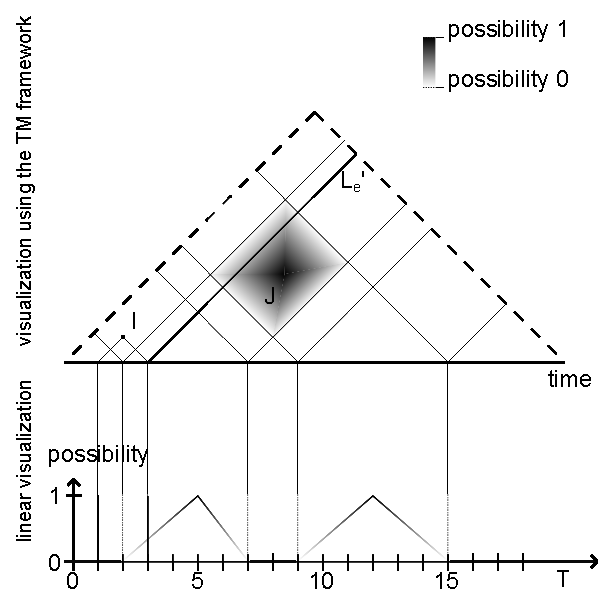
\includegraphics[width=0.9\columnwidth]{graphs/example_image.eps}
	\caption{The visualization of the example using the TM framework.}
	\label{fig:ex}
\end{figure}
 
%We will illustrate the calculation of one Allen Relation with an example.
%\begin{example}
%Consider a CTI $J = [1, 3]$ the two ill-known time points $S, E$ that define a time interval. 
%We want to obtain the possibility that $J$ is before the time interval.
%The points are defined by two triangular membership functions $\mu_S$, $\mu_E$.

%\begin{align}
%\label{eq:ex-point}
%\pi_S &= \mu_S = \left[2,5,7 \right] \\
%\pi_E &= \mu_E = \left[9,12,15 \right]
%\end{align}

%Then, it is possible to define both an IKTI $I$ Eq. \eqref{eq:ex-uti-ikti} and an UTI $\pi_I$ Eq. \eqref{eq:ex-uti-uti}. The intervals are illustrated in Figure \ref{fig:example}.

%\begin{figure}[h]
%   \centering
%   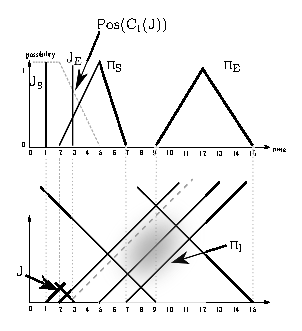
\includegraphics[scale=1.5]{graphs/example.eps}
%   \caption{In the top, the crisp time interval $J$ and the IKTI given by $I = [S, E]$. The ill-known constraint for the before relation is illustrated in grey color. In the lower graphic, the interval point $J$ and the UTI $\pi_I$. }
%   \label{fig:example}
% \end{figure}

%\begin{align}
%\label{eq:ex-uti-ikti}
%I = \left[S, E \right]\\
%\label{eq:ex-uti-uti}
%\mu_I = \left(\mu_S, \mu_E \right)
%\end{align}

%First we will obtain the possibility between $J$ and the UTI $\pi_I$. The relation possibly meets has three candidates: Before, Meets and Overlaps.

%\begin{align}
%  \mu_{\left(J R \pi_I \right)}(B) &= \sup_{a < e} \pi_S(a)\\
%\mu_{\left(J R \pi_I \right)}(M) &= \pi_S(e)\\
%\mu_{\left(J R \pi_I \right)}(O) &= \sup_{a > e} \pi_S(a)
%\end{align}

%\begin{align}
%\mu_{\left(J R \pi_I \right)}(B) &= 0.67\\
%\mu_{\left(J R \pi_I \right)}(M) &= 0.33\\
%\mu_{\left(J R \pi_I \right)}(O) &= 0
%\end{align}

%In order to compute the possibility  for the before relation between the crisp interval $J$ and the IKTI $I$, a ill-known constraint is needed.

%\begin{equation}
% C_1\stackrel{\triangle}{=} \left(<,X\right)
%\end{equation}

%Then the possibility is computed as follows:

%\begin{align}
%\Pos \left(C_1 (J) \right) &= \sup_{a < e} \pi_S(a)\\
%\Pos \left(C_1 (J) \right) &= 0.67 
%\end{align}






%\end{example}



% 
% In this section we will analyze first the calculation of all the possible Allen's relations between a crisp time point and an ill-known time point and between a crisp time point and an uncertain time indication (UTI). Then, we will compare two ill-known time points and two uncertain time indications.

% \subsection{\label{subsec:prop-crisp-vs-ill}Calculation of crisp time intervals}
% In this section we first study how uncertainty about wheter crisp interval is enclosed by the ill-known interval given by $[X,Y]$ or by the UTI.
% 
% \subsubsection{Crisp time interval enclosed by an ill-known time interval}
% Consider a crisp time interval given by $I=[a, b]$. We want to know whether all the points in this interval are within the boundaries of the ill-known interval given by $[X, Y]$. The calculation is done by means of two ill-known constraints as explained in \cite{}:
% \begin{eqnarray}
% C_1\stackrel{\triangle}{=}\left(\geq,X\right)\\
% C_2\stackrel{\triangle}{=}\left(\leq,Y\right).
% \end{eqnarray}
% 
% The possibility and the necessity are given by:
% \begin{eqnarray}
% \Pos\left(\lambda([a,b])\right)&=&\min\bigg(\Pos(C_1([a,b])),\Pos(C_2([a,b]))\bigg)\\
% \Nec\left(\lambda([a,b])\right)&=&\min\bigg(\Nec(C_1([a,b])),\Nec(C_2([a,b]))\bigg).
% \end{eqnarray}
% Which can be expanded to:
% \begin{eqnarray}
% \label{eq:interval-pos}
% \Pos\left(\lambda([a,b])\right)&=&\min\bigg(\sup_{a\leq w}\pi_{X}(w),\sup_{b\geq w}\pi_{Y}(w)\bigg)\\
% \label{eq:interval-nec}
% \Nec\left(\lambda([a,b])\right)&=&\min\bigg(\inf_{a>w}1-\pi_{X}(w),\inf_{b<w}1-\pi_{Y}(w)\bigg).
% \end{eqnarray}
% 
% 
% \subsubsection{\label{subsubsec:crisp-uti}Crisp time interval enclosed by an UTI}
% Consider now a crisp time interval given by $I=[a, b]$ and an Uncertain Time Interval given by $\pi_I = \left(\pi_s, \pi_e \right)$. Again, we want to know if all the points in the interval are within the boundaries of the UTI. The calculation is done as explained in \cite{}:
% \begin{equation}
%  \pi_I \left( \left[a, b  \right] \right) =
% \begin{cases}
%  \min \left(\pi_s(a),\pi_e(b)\right) & \mbox{ if } a \leq b\\
% 0 				     & \mbox{ otherwise. }
% \end{cases}
% \end{equation}

%Two frameworks for dealing with uncertainty in time intervals have been presented. In this section, we will study the equivalences between an uncertain time interval (UTI) and an ill-known time interval (IKTI). Nevertheless, there are some differences in the semantics of UTIs and IKTIs which are also explained. Next to that, the computation of the Allen's Relations are compared.

%\subsection{\label{subsec:sim-dif}Similarities and differences}
%A time interval is defined by a starting and an ending point. When uncertainty arises, in one or both starting and / or ending points, then either an UTI $\pi_I$ or an IKTI can be used. 

%\begin{itemize}
% \item An IKTI $J = \left[X, Y \right]$ is defined by two ill-known values $X, Y$ which are respectively, the starting and ending points of the time interval. Two possibility distributions $\pi_X, \pi_Y$ are defined for $X$ and $Y$ respectively.
%\item An UTI $\pi_I$ is defined by two possibility distributions, $\pi_S$, $\pi_E$ for the starting  and ending point respectively.
%\end{itemize}

%In the following, we will assume that:

%\begin{align}
%\pi_X &= \pi_S = \mu_S \\
%\pi_Y &= \pi_E = \mu_E
%\end{align}

%Where $\mu_S, \mu_E$ are triangular membership functions. Notice that the main difference between an UTI and an IKTI is a matter of interpretation. IKTIs  keep both possibility distributions for both starting and ending points, while UTIs take a t-norm (the minimum) of both possibility distributions (see Eq. \eqref{eq:possibility-uti}). That is, not all the crisp intervals between the boundaries of the starting and ending point are candidate intervals for the UTI.

%\begin{figure}[h]
%   \centering
%   
\includegraphics[scale=1.5]{graphs/equivalences.eps}
%   \caption{Possibility degrees for two candidate intervals with respect to the UTI $\pi_I$. The upper crisp time interval has a possibility degree of 1, whereas the lower crisp interval has a possibility degree of 0. }
%   \label{fig:ikc-greater}
% \end{figure}

%It is possible to obtain the same interpretation for an IKTI, but some ill-known constraints must be defined over the starting and ending ill-known values $X$, $Y$. In \cite{Pons2011}, two constraints are defined to determinate whether a crisp time interval $[a, b]$ resides between the boundaries of $J$. In this case, all the crisp intervals whose boundaries are within the boundaries of $X$ and $Y$ are considered to be a candidate interval. Nevertheless, if we want to obtain the same interpretation as in the UTI, the following two ill-known constraints must be defined:

%\begin{align}
% \label{eq:ikc-ikti-uti}
%C_1 &\triangleq \left(=, X \right) \\
%C_2 &\triangleq \left(=, Y \right)\\
%\Pos \left(\left[a, b\right] \right) &= C_1 \left(a \right) \wedge C_2\left(b \right) =\\
%\label{eq:equivalence-ikti-uti}
%\Pos \left(\left[a, b\right] \right) &= \min \left( \pi_X(a), \pi_Y(b) \right)
%\end{align}

%In this case, Eq. \eqref{eq:equivalence-ikti-uti} is equivalent to Eq. \eqref{eq:possibility-uti}.
%In the following subsection, we will study the connection between the Allen's relations in each framework.

%\subsection{\label{subsec:eval-allen-relations}Evaluation of the Allen's Relations}
%As it has been shown in Table \ref{tab:urz}, when using UTIs in the triangular model, it is possible to obtain a more detailed relational information (there are fifteen possible relations) than with the ill-known constraint approach. The following observations should be taken into account when extracting relational information from both frameworks:

%\begin{itemize}
% \item In TM, the Allen's Relations $R \in \left \lbrace B, O, C, D, OB, A \right \rbrace$ between an interval point $J$  and an UTI $\pi_I$ are computed by Eq. \eqref{eq:possibility-iz-uti-certain}. Therefore, for the Allen's Relations in $R$, 
% possibility that an Allen Relation between an interval point $J$  and an UTI $\pi_I$ is $1$ if the interval point $J$ is in the Allen Relation, or $0$ in other case.
%\item In the TM, the other nine Allen's Relations between an interval point $J$ and an UTI $\pi_I$ are graded from $1$ to $0$ and computed by using the Eq. \eqref{eq:possibility-iz-uti}. 
%\item In the ill-known constraint framework, all the thirteen Allen's Relations are computed by using an aggregation of ill-known constraints (see Table \ref{tab:allen-relations}). Therefore, the possibility that a time point $J$ is in a given Allen Relation is always graded from $1$ to $0$.
%\end{itemize}

%For example, consider that we want to know whether the relation Before (B) holds between a time point $J$ and an IKTI $I$. We will note $\Pos \left(C_B (J)  \right)$ the possibility that the relation before holds. There are three possibilities:
%\begin{enumerate}
% \item $\Pos \left(C_B (J)  \right)$ = 1: The time point $J$ is before the IKTI $I$.
%\item $\Pos \left(C_B (J)  \right)$ = 0: The time point $J$ is not before the IKTI $I$.
%\item $0 < \Pos \left(C_B (J)  \right) < 1$: The time point $J$ is to some extent before the IKTI $I$.
%\end{enumerate}

%The last case corresponds in the TM to case when the before relation is one of the possible relations (See Table \ref{tab:urz}). That is, one of $\left \lbrace PM, PMB, UB \right \rbrace$.

%The following table establishes the correspondences between the Allen's relations in the TM and in the ill-known constraints framework.




%\begin{table}[h]
%\centering
%\begin{tabular}{|l|l|l|}
%\hline
%Symbol & Name & Possible Relations \\
%\hline
%B & Before & B, PM, PMB, UB \\
%\multirow{2}{*}
%{O} & Overlaps & O, PM, PS, PFB,\\
%     &          &  PE, PMB, UB \\
%C & Contains & C, PFB, PE, PSB \\
%\multirow{2}{*}
%D & During & D, PS, PE, \\
%  &         &  PMB, UB  \\
%OB & Overlapped by & OB, PE, PSB, PF \\
%A & After & A, PF, UE \\
%M & Meets & M, PM, PMB, UB \\
%MB & Met By & MB, PF, UE \\
%E & Equals & E, PE \\
%\multirow{2}{*}
%S & Starts & S, PS, PE, \\
%  &         &   PMB, UB \\
%SB & Started by & SB, PE, PSB \\
%F & Finishes & F, PE \\
%FB & Finished By & FB, PE, PFB\\
%\hline
%\end{tabular}
%\caption{Correspondences between the Allen's Relations in the ill-known constraint framework and the triangular model,}
%\label{tab:correspondences-tm-ikcf}
%\end{table}